\documentclass[reportComp]{thesis}
\usepackage[cpp,linenum]{mypackage}

\title{数值计算方法实验报告}
\subtitle{实验一:插值多项式}
\school{数据科学与计算机学院}
\author{陈鸿峥}
\classname{17大数据与人工智能}
\stunum{17341015}
\headercontext{数值计算方法实验报告}

\begin{document}

\maketitle

\section{题目描述}
\begin{itemize}
    \item 使用区间$[-5,5]$上的21个等距节点,找出函数$f(x)=(x^2+1)^{-1}$的20阶插值多项式$p(x)$。
    打印出$f(x)$和$p(x)$的图形,观察$f(x)$和$p(x)$的最大偏差。
    \item 在计算机上,对上一题使用切比雪夫节点$x_i=5\cos(i\pi/20),0\leq i\leq 20$,找出函数$f(x)=(x^2+1)^{-1}$的20阶插值多项式$q(x)$。
    打印出$f(x)$和$q(x)$的图形,由上一题和本题,你能得出什么结论?
\end{itemize}

\section{实验结果与分析}
采用Wolfram Mathematica 11.1进行编程实验,实验结果如图\ref{fig:px}和图\ref{fig:qx}所示。
由于$p(x)$函数波动太大,故在图\ref{fig:px}的左图中仅仅显示了$[-4,4]$的区间。
\begin{figure}[H]
\centering
\begin{tabular}{cc}
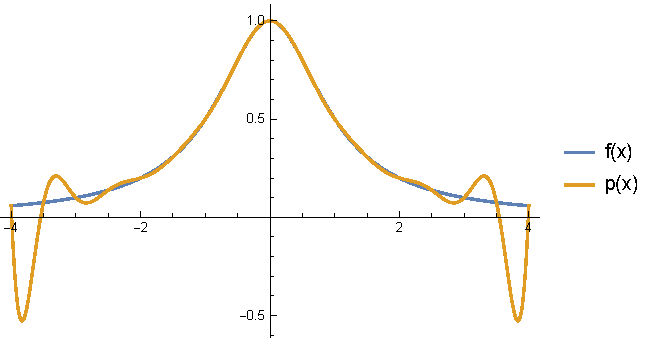
\includegraphics[width=0.5\linewidth]{px.pdf}&
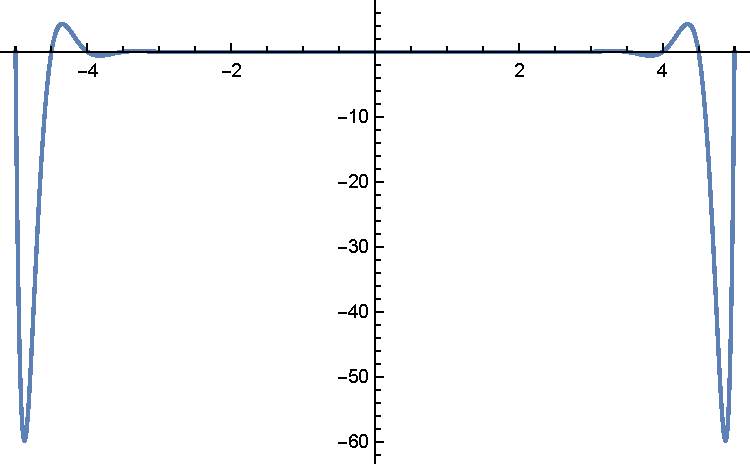
\includegraphics[width=0.5\linewidth]{px-err.pdf}
\end{tabular}
\caption{$f(x)$与$p(x)$的图形与误差}
\label{fig:px}
\end{figure}
\begin{figure}[H]
\centering
\begin{tabular}{cc}
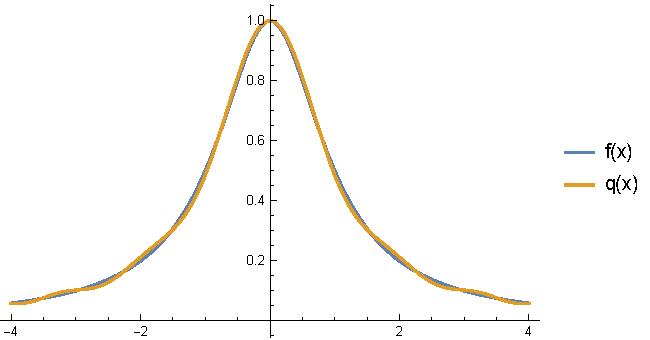
\includegraphics[width=0.5\linewidth]{qx.pdf}&
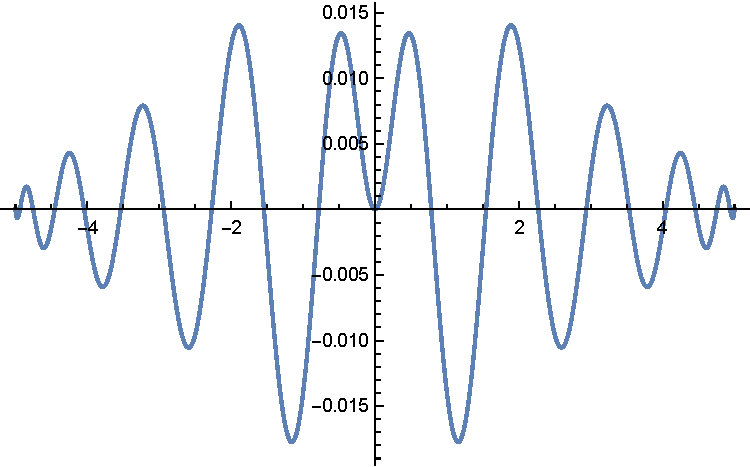
\includegraphics[width=0.5\linewidth]{qx-err.pdf}
\end{tabular}
\caption{$f(x)$与$q(x)$的图形与误差}
\label{fig:qx}
\end{figure}

由图\ref{fig:px}可以看出,$p(x)$在$[-2,2]$的区间都拟合得比较好,与$f(x)$的绝对误差接近于$0$;
而在大约$\pm 4.8$的位置,误差达到最大,绝对误差接近于$60$。

由图\ref{fig:qx}则可以看出,$q(x)$在$[-5,5]$整个区间上都拟合得很好,最大绝对误差也不超过$0.02$,进而得出结论:在本题的插值函数中采用切比雪夫节点会获得比较好的效果(即误差较小)。

证明由课本下一章切比雪夫多项式的性质可得。
设切比雪夫多项式为$T_n(x)=\cos(n\cos^{-1}(x))$,有零点$x_i=\cos\lrp{\dfrac{(2i-1)\pi}{2n}},i=1,\ldots,n$,进而
\[T_n(x)=2^{n-1}\prod_{i=0}^n(x-x_i)\]
若在$[-1,1]$上进行拉格朗日插值,则余项为
\[|R_n(x)|=|f(x)-q(x)|=\lrabs{\frac{f^{(n+1)}(\xi)}{(n+1)!}\prod_{i=0}^{n}(x-x_i)}\]
其中$\xi\in(-1,1)$。
记$M_{n+1}=\max_{x\in[-1,1]}|f^{(n+1)}(x)|$,则
\[|R_n(x)|\leq\frac{M_{n+1}}{(n+1)!}\max_{x\in[-1,1]}\lrabs{\prod_{i=0}^{n}(x-x_i)}=\frac{M_{n+1}}{(n+1)!}\max_{x\in[-1,1]}\lrabs{\frac{T_{n+1}(x)}{2^n}}=\frac{M_{n+1}}{(n+1)!2^n}\]
可见误差非常小。
若将区间换为$[-5,5]$,同理可得
\[|R_{n}(x)|\leq \frac{5^n\max_{x\in[-5,5]}|f^{(n+1)}(x)|}{(n+1)!2^n}\]

\section{源代码}
下面为本次实验的Mathematica源代码,完整文件已在附件中\verb'interpolation.nb'。
注意下列插值函数均为自己编写,没有调用系统库函数。
\begin{lstlisting}[language=mathematica]
f[x_] := (x^2 + 1)^(-1)
px = Array[# &, 21, {-5, 5}];(*equal length*)
px2 = Table[N[5 Cos[i \[Pi]/20]], {i, 0, 20}]; (*Chebyshev*)
(*My Lagrange function, not using InterpolatingPolynomial*)
l[px_] := 
 Sum[Product[If[j != i, x - px[[j]]], {j, 1, 21}]/
   Product[If[j != i, px[[i]] - px[[j]]], {j, 1, 21}] f[px[[i]]], {i, 
   1, 21}];
Plot[{Legended[f[x], "f(x)"], Legended[l[px], "p(x)"]}, {x, -4, 4}]
Plot[l[px] - f[x], {x, -5, 5}, PlotRange -> Full]
Plot[{Legended[f[x], "f(x)"], Legended[l[px2], "q(x)"]}, {x, -4, 4}]
Plot[l[px2] - f[x], {x, -5, 5}]
\end{lstlisting}

\end{document}
% 1024180018@qq.com
% shuzhijisuan2017@163.com

% 上机作业要求
% 建议使用C++/Matlab编程,注:不允许使用内置函数完成主要功能
% 主题/文件名:班级+姓名(小组)+学号+第几次作业
% 实验报告(运行结果)、源代码